\chapter{Representació de camps} \label{ch:informe 1}
\begin{resum}
	L'objectiu principal d'aquesta pràctica consisteix en representar les línies de camp elèctric i línies equipotencials degudes a tres distribucions de càrrega: un condensador de plaques plano-para\l.leles, dos fils infinits i para\l.lels i una altra distribució lliure, amb la qual vam estudiar l'efecte punxa. A més, vam analitzar la capacitat del condensador trobant la càrrega per unitat de longitud.

	Els resultats han estat acurats als dos primer casos, trobant representacions molt semblants a les teòriques. La capacitat del condensador ha estat de $C/\epsilon = \data{1.6}{0.4}{F.m^{-1}} $, resultat molt proper al teòric. La distribució lliure no ens ha permès estudiar l'efecte que volíem, però hem observat l'importància de les dimensions a les distribucions de càrrega.
\end{resum}

\section{Introducció}
Sabem que existeixen materials als que el camp elèctric\footnote{A partir d'ara, si diem \textit{camp}, ens estarem referint a aquest camp} $\vec{E}$ està relacionat amb la densitat de corrent $\vec{J}$ i amb el vector desplaçament $\vec{D}$ mitjançant únicament una constant numèrica. D'aquesta manera, en medis lineals, isòtrops i homogenis, es compleix que si el rotacional del camp elèctric és nul, com és en l'aproximació electrostàtica, aleshores també ho són els rotacionals de $\vec{J}$ i $\vec{D}$. Així, tots tres poden ser deduïts a partir d'un potencial tal que compleixi l'equació de Laplace. Això és prou útil en tant que ens permet conèixer automàticament la solució d'un problema en un medi conductor si coneixem la resolució en un dielèctric i viceversa. Aquest fenomen ens permetrà representar línies equipotencials produïdes per distribucions de càrrega en les que hi ha alguna mena de simetria.

Considerem doncs una d'aquestes situacions amb simetria, la de dues plaques plano-para\l.leles d'un condensador. Si, enlloc de plantejar el problema en tres dimensions, escollim una superfície plana tal que talli perpendicularment les plaques, podem estudiar la relació entre càrrega, diferència de potencial i capacitat d'un condensador de manera anàloga. Si definim ara $Q/Z$ com la càrrega d'una de les plaques per unitat de longitud i $V_a-V_b$ com la diferència de potencial entre les plaques, tenim que la capacitat per unitat de longitud $C/Z$ ve donada per
\begin{equation} \label{eq:capacitat}
	C/Z=\frac{Q/Z}{V_a-V_b}
\end{equation}

D'altra banda, els objectius d'aquesta pràctica seran estudiar les línies equipotencials i de camp per a diferents distribucions de càrrega: dues plaques plano-para\l.leles d'un condensador i dos fils infinits para\l.lels. Així mateix, haurem de calcular la capacitat per unitat de longitud d'un condensador de plaques plano-para\l.leles.I per últim estudiarem l'efecte punxa comparant dues superfícies de curvatures diferenciades.
\end{itemize}
\section{Mètode experimental}
Com comentàvem, suposem que les distribucions de càrrega del condensador i els dos fils tenen longitud a la component $z$ infinita, de manera que qualsevol pla para\l.lel al nostre pla, diguem-li $xy$, seria igual al que tenim. Per al cas adicional de l'efecte punxa, suposem simetria al voltant de l'eix $x$ del paper: qualsevol pla que el contingui com a eix d'abcises hauria de ser igual al nostre. Utilitzarem un paper impregnat de carbó i amb conductivitat uniforme per a dibuixar les distribucions de càrrega mitjançant un retolador de tinta de plata amb una conductivitat més gran que la del paper. 

A l'hora de la realització experimental, primer cal dibuixar la distribució que convingui i deixar que la tinta s'assequi. Un cop fixat el muntatge de la \cref{fig:muntatge}, connectem cada placa (element del dibuix) a una entrada de la font.Connectem també un dels electrodes a un dels cables del multímetre, que servirà de referència de potencial. Mitjançant l'altre extrem del multímetre, mesurem el potencial en qualsevol punt del paper simplement tocant amb la punxa el punt que sigui. 

Després hem de dibuixar línies equipotencials buscant punts amb el mateix potencial. Les línies de camp es troben posteriorment, aprofitant que són perpendiculars a les línies equipotencials. Per al cas particular del condensador, la determinació de la càrrega per unitat de longitud vindrà donada per l'\cref{eq:carrega}, on apareixen la diferència de potencial entre dos punts de les superfícies equipotencials ($\Delta V_i$), la distància radial que les separa mesurada sobre la línia de camp elèctric
		($\Delta r_i$) i la separació longitudinal entre dos punts consecutius a la mateixa superfície equipotencial ($\Delta l_i$), així com la permitivitat elèctrica del medi.
		\begin{equation}\label{eq:carrega}
			Q/Z=\epsilon \sum_i \frac{\Delta V_i \Delta l_i}{\Delta r_i}
		\end{equation}
I per a comparar amb el valor teòric de la capacitat, s'ha de fer servir l'expressió \cref{eq:capacitat 2}, que relaciona longitud de la component $y$ de les plaques ($h$), separació ($d$) i la permitivitat  $\epsilon$ del medi.
		\begin{equation}\label{eq:capacitat 2} 
			C/Z=\frac{h}{d}\epsilon
		\end{equation}

Addicionalment es va simular el potencial de cada una de les tres distribucions considerades mitjançant l'algoritme de Jacobi ---els codis són als \cref{lst:condensador,lst:fils,lst:lliure}---.

\begin{figure}[htb]
	\centering
	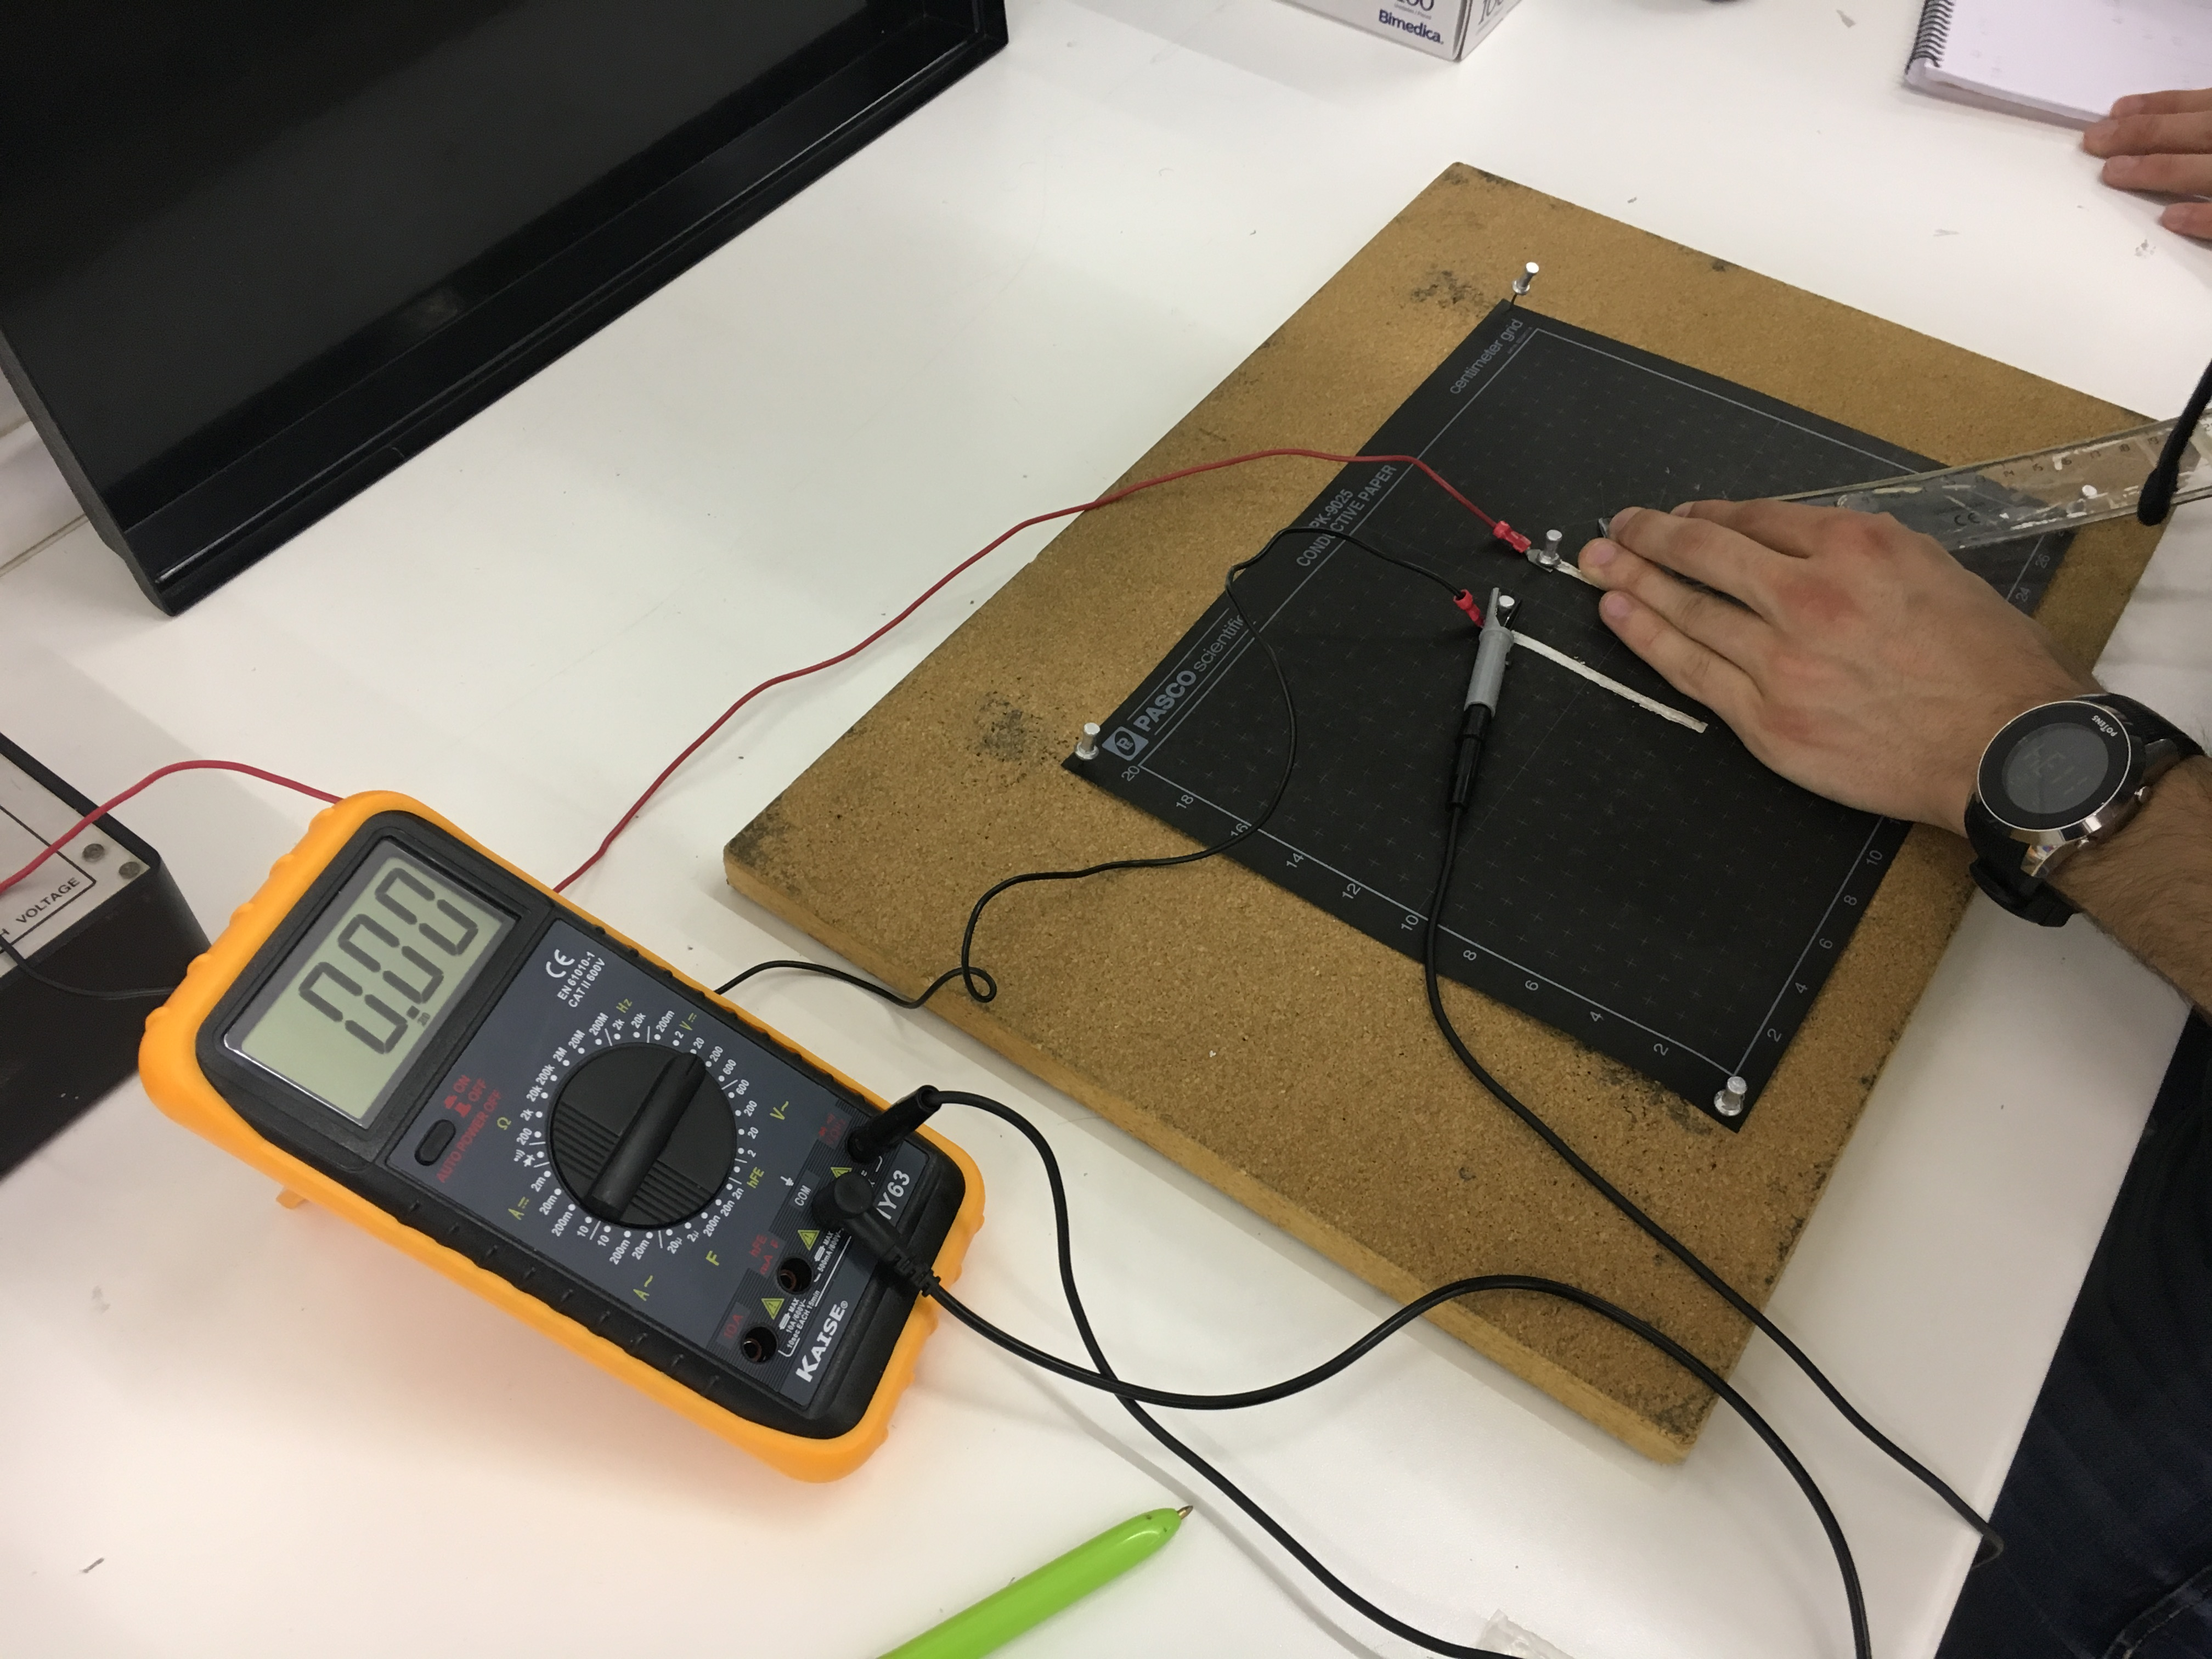
\includegraphics[scale=0.05]{muntatge-camps.JPG}
	\caption{Muntatge experimental}
	\label{fig:muntatge}
\end{figure}

\section{Resultats}
El nostre objectiu és representar qualitativament les línies equipotencials produïdes per diferents distribucions de càrrega. Principalment ens centrarem en la forma, però també ens interessa el valor del potencial associat a cada línia, o el valor de la diferència de potencial entre la distribució i la línia, més precisament. En tots els casos, hi fixarem una diferència de potencial de \SI{9}{V}. Els punts mesurats tenen una incertesa associada de \data{}{0.02}{V}, degut a la suma de voltatges. I a més hem realitzat algunes simulacions per a comprovar resultats en tant que forma, però no pas en valors degut a les condicions de contorn. A les \cref{fig:carbo condensador,fig:carbo fils} i a la \cref{fig:carbo lliure} es poden apreciar els papers de carbó ja mencionats i les distribucions de càrrega, acolorides de plata.

\begin{figure}[htb]
  \centering
	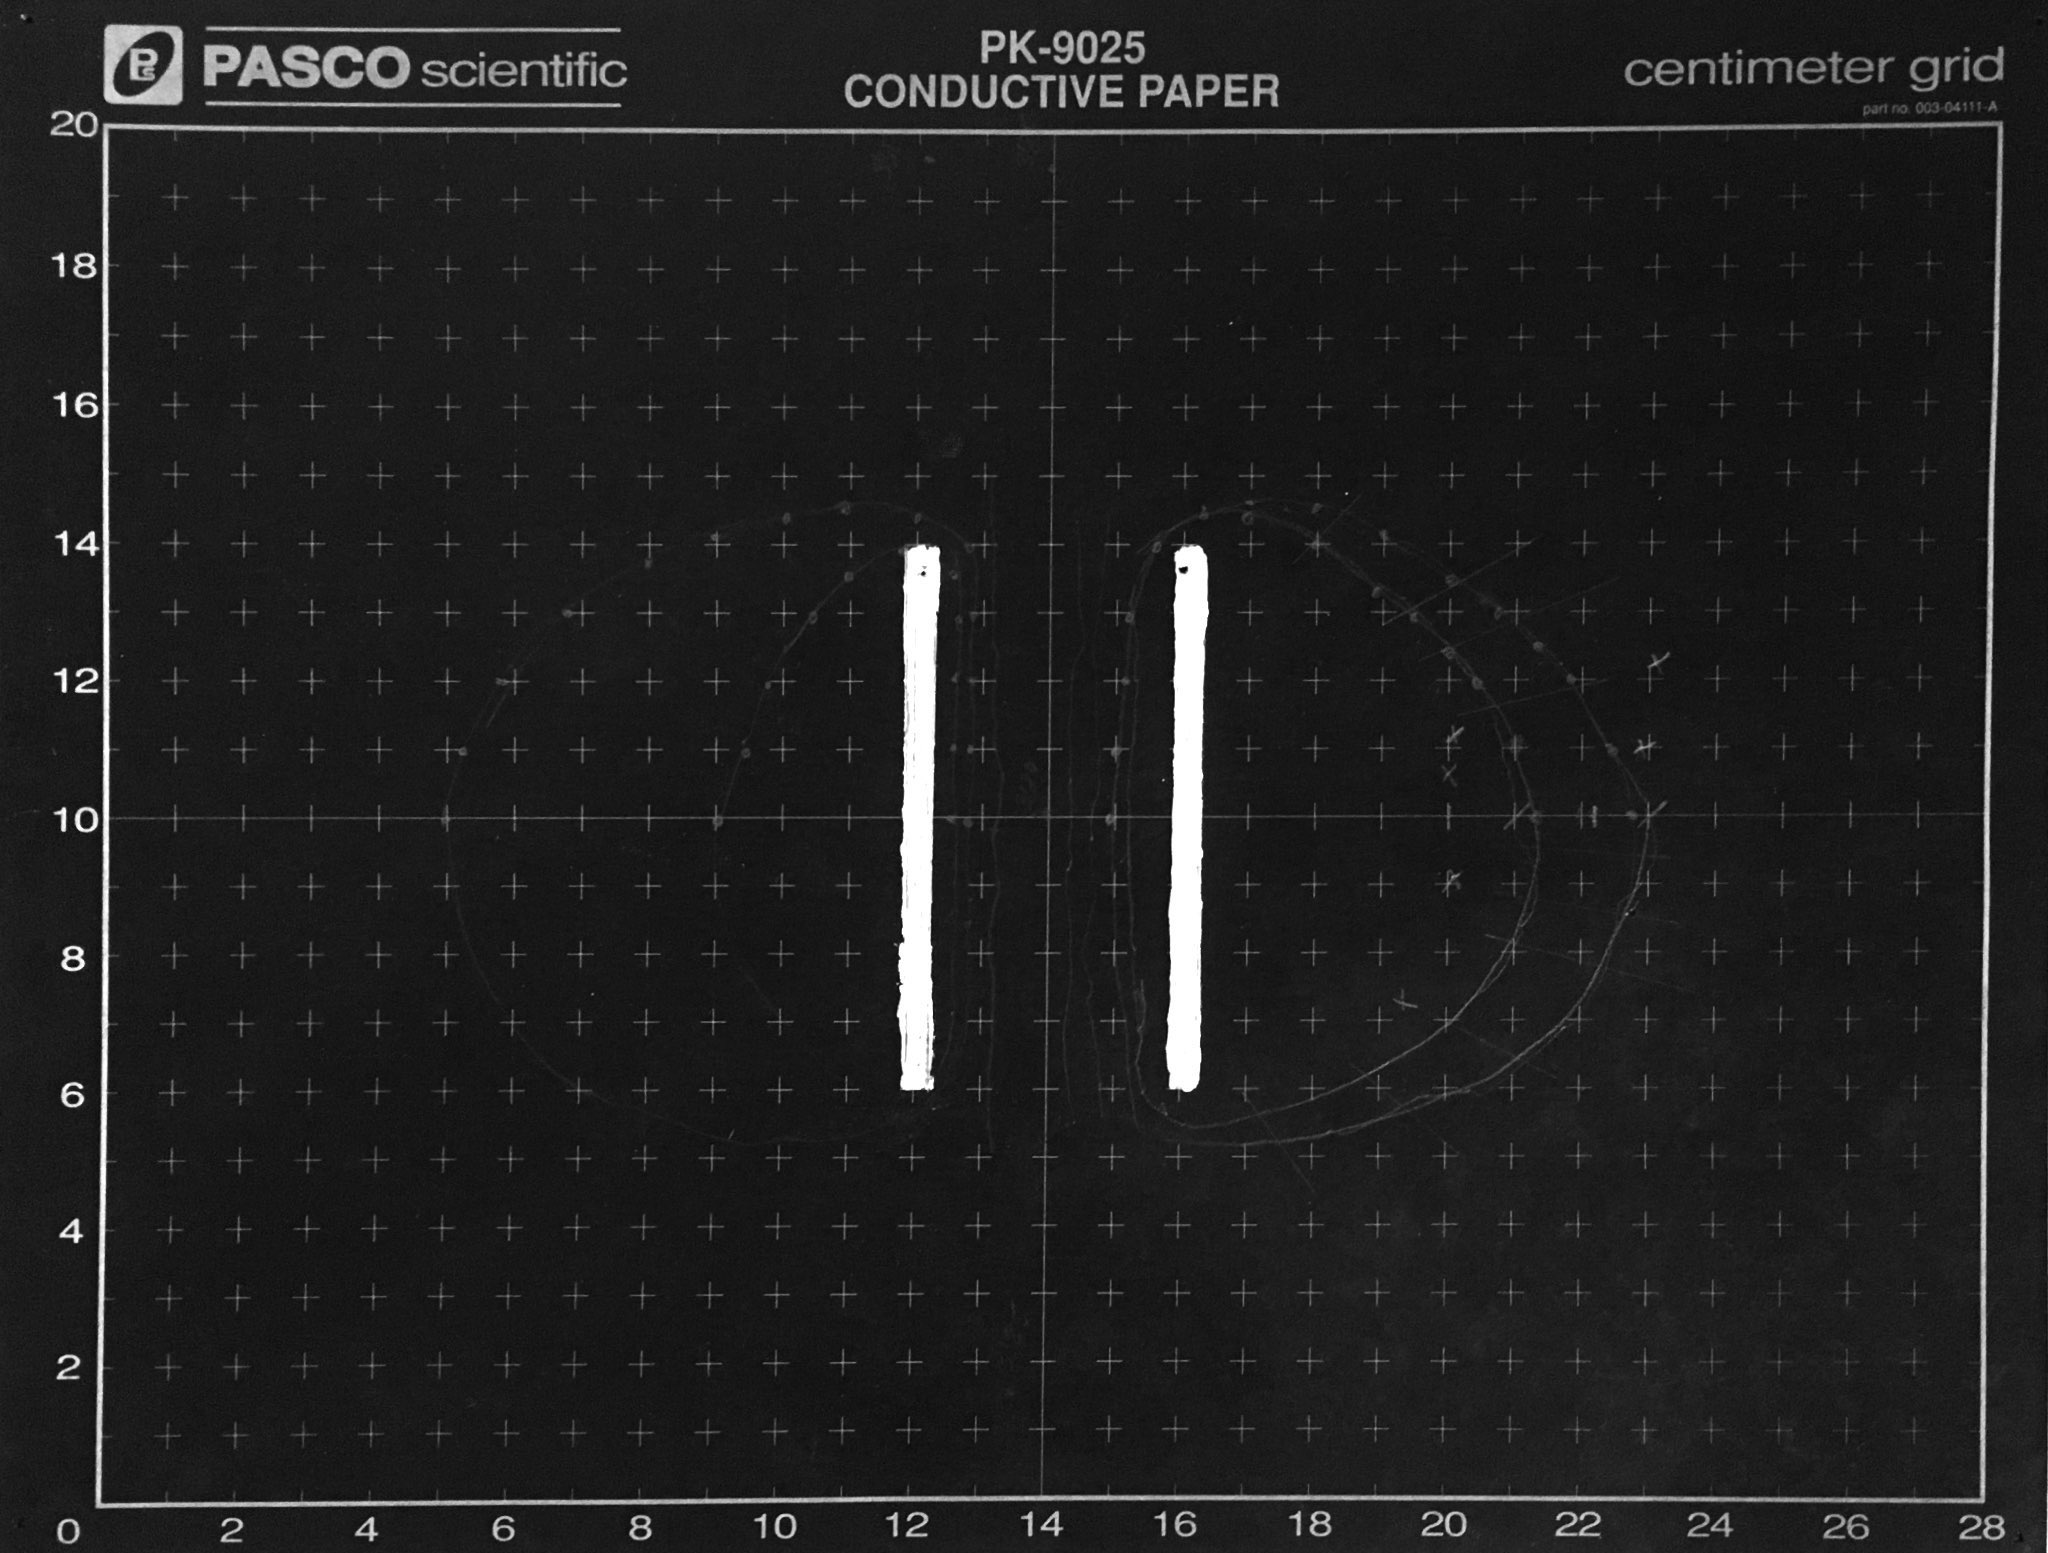
\includegraphics[scale=0.1]{carbo-condensador.jpg}
  \caption{Paper de carbó corresponent al condensador}
  \label{fig:carbo condensador}
\end{figure}

\begin{figure}[htb]
  \centering
	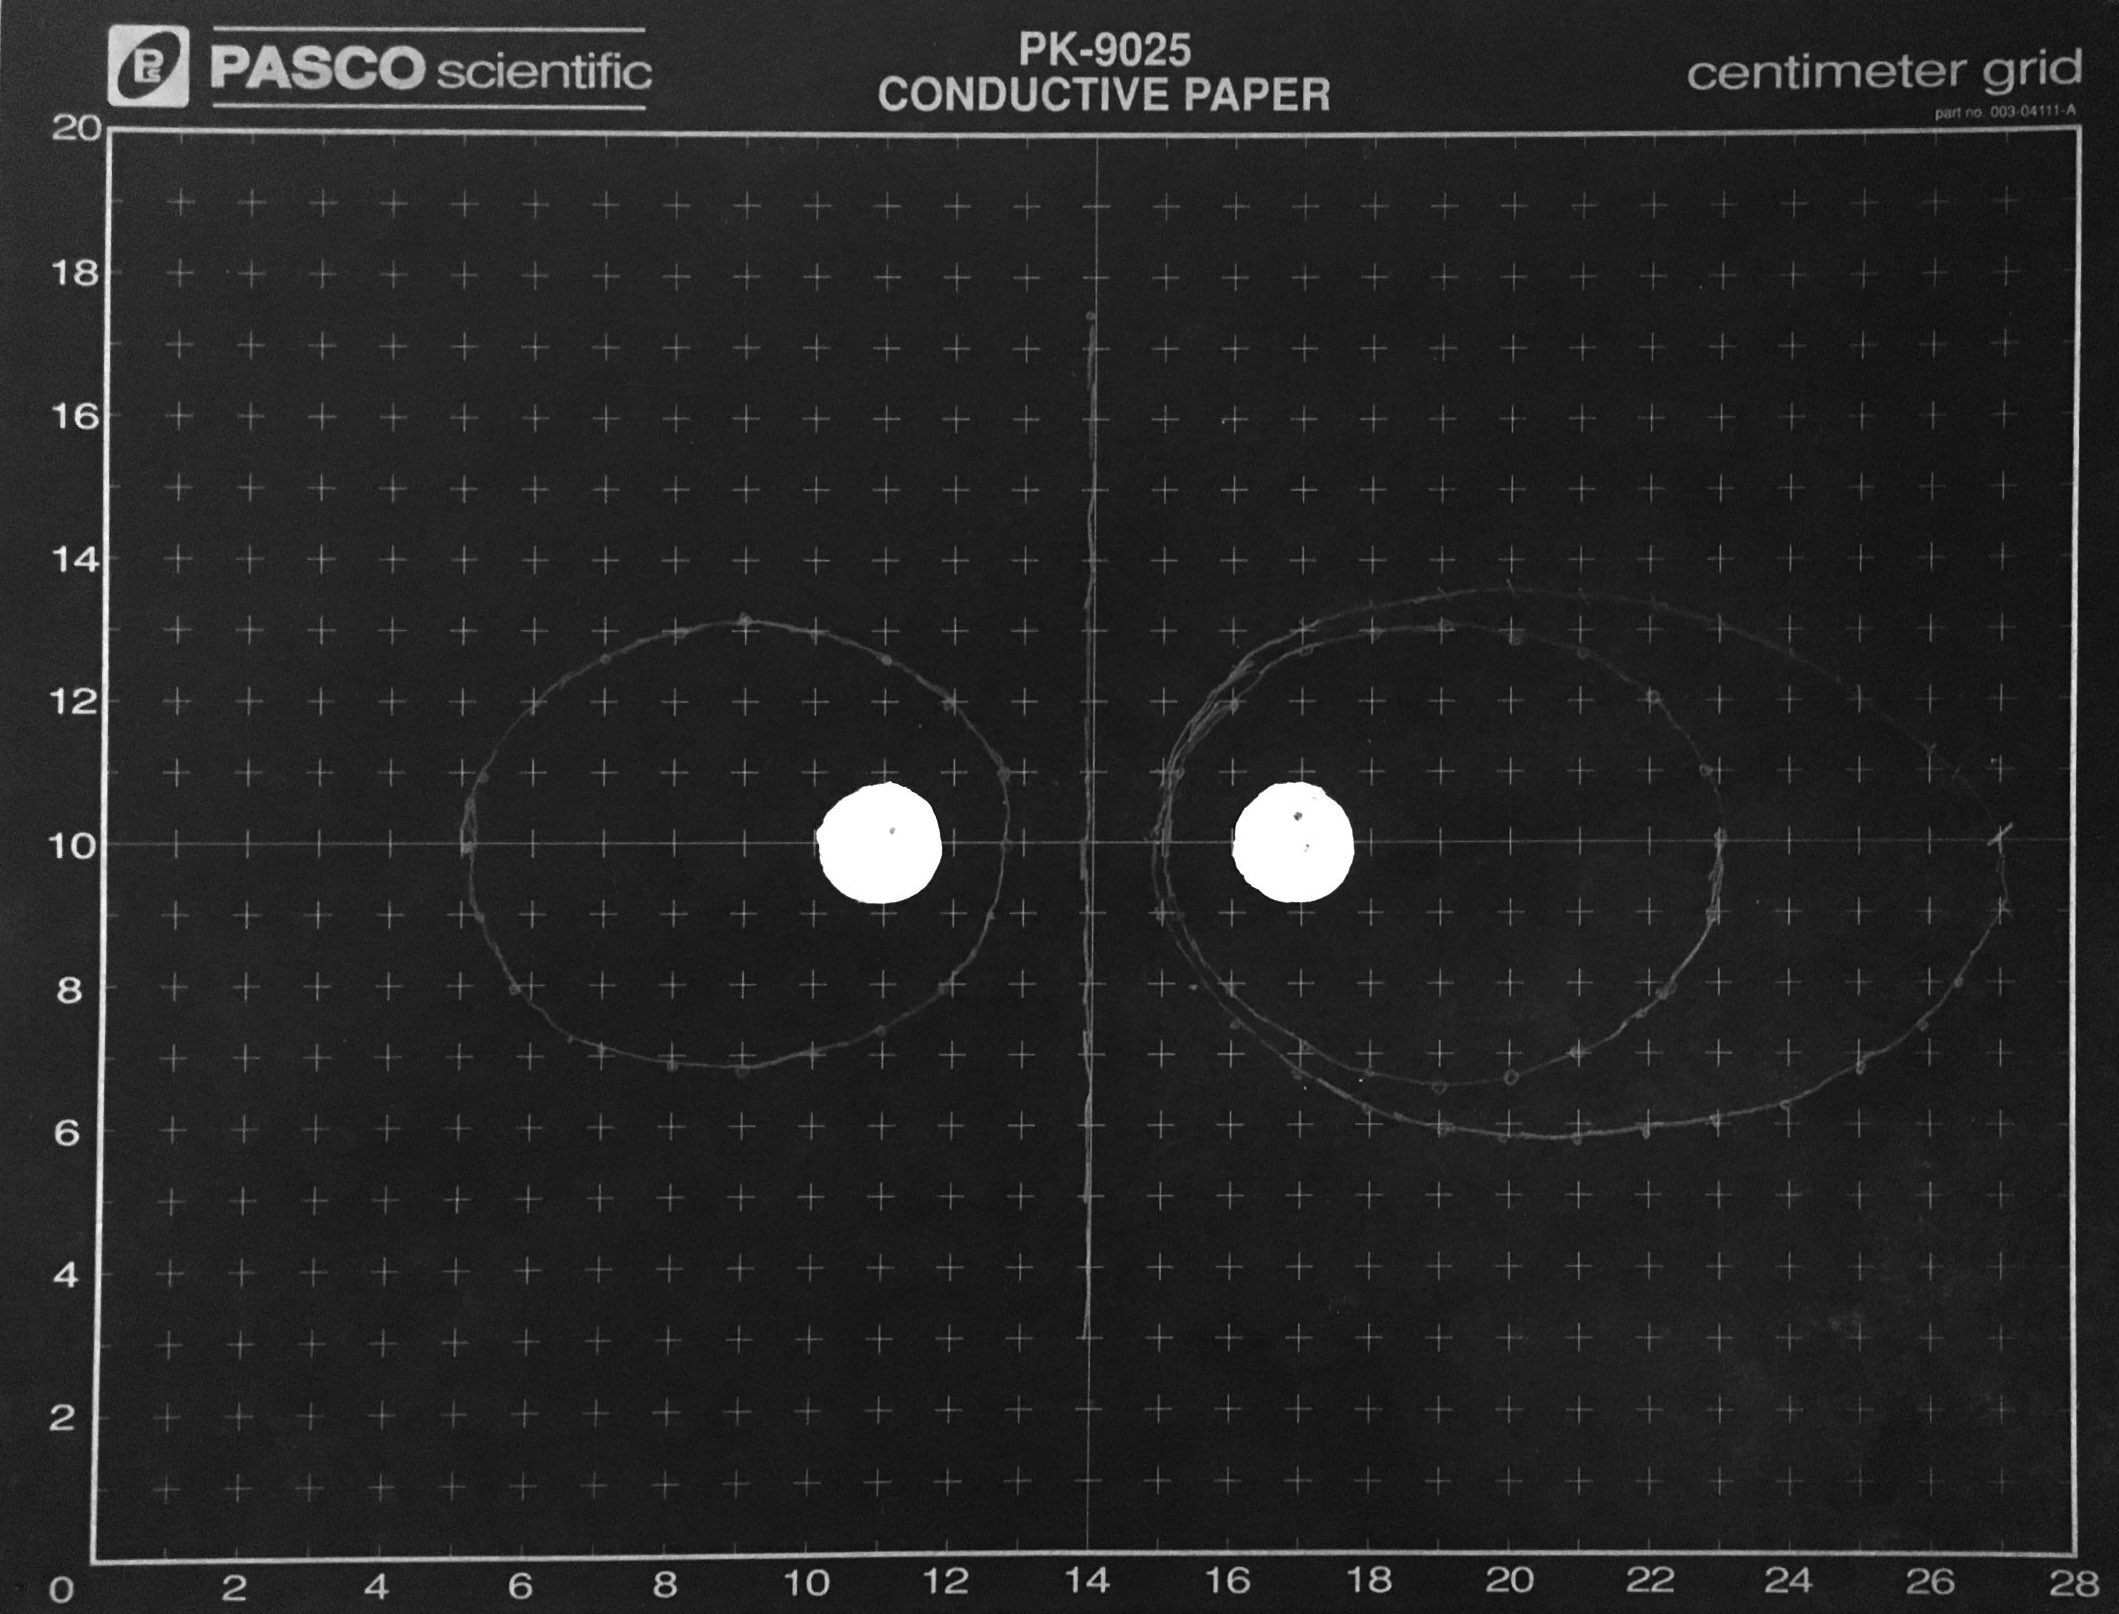
\includegraphics[scale=0.1]{carbo-fils.jpg}
  \caption{Paper de carbó corresponent als fils para\l.lels}
  \label{fig:carbo fils}
\end{figure}

\begin{figure}[htb]
  \centering
	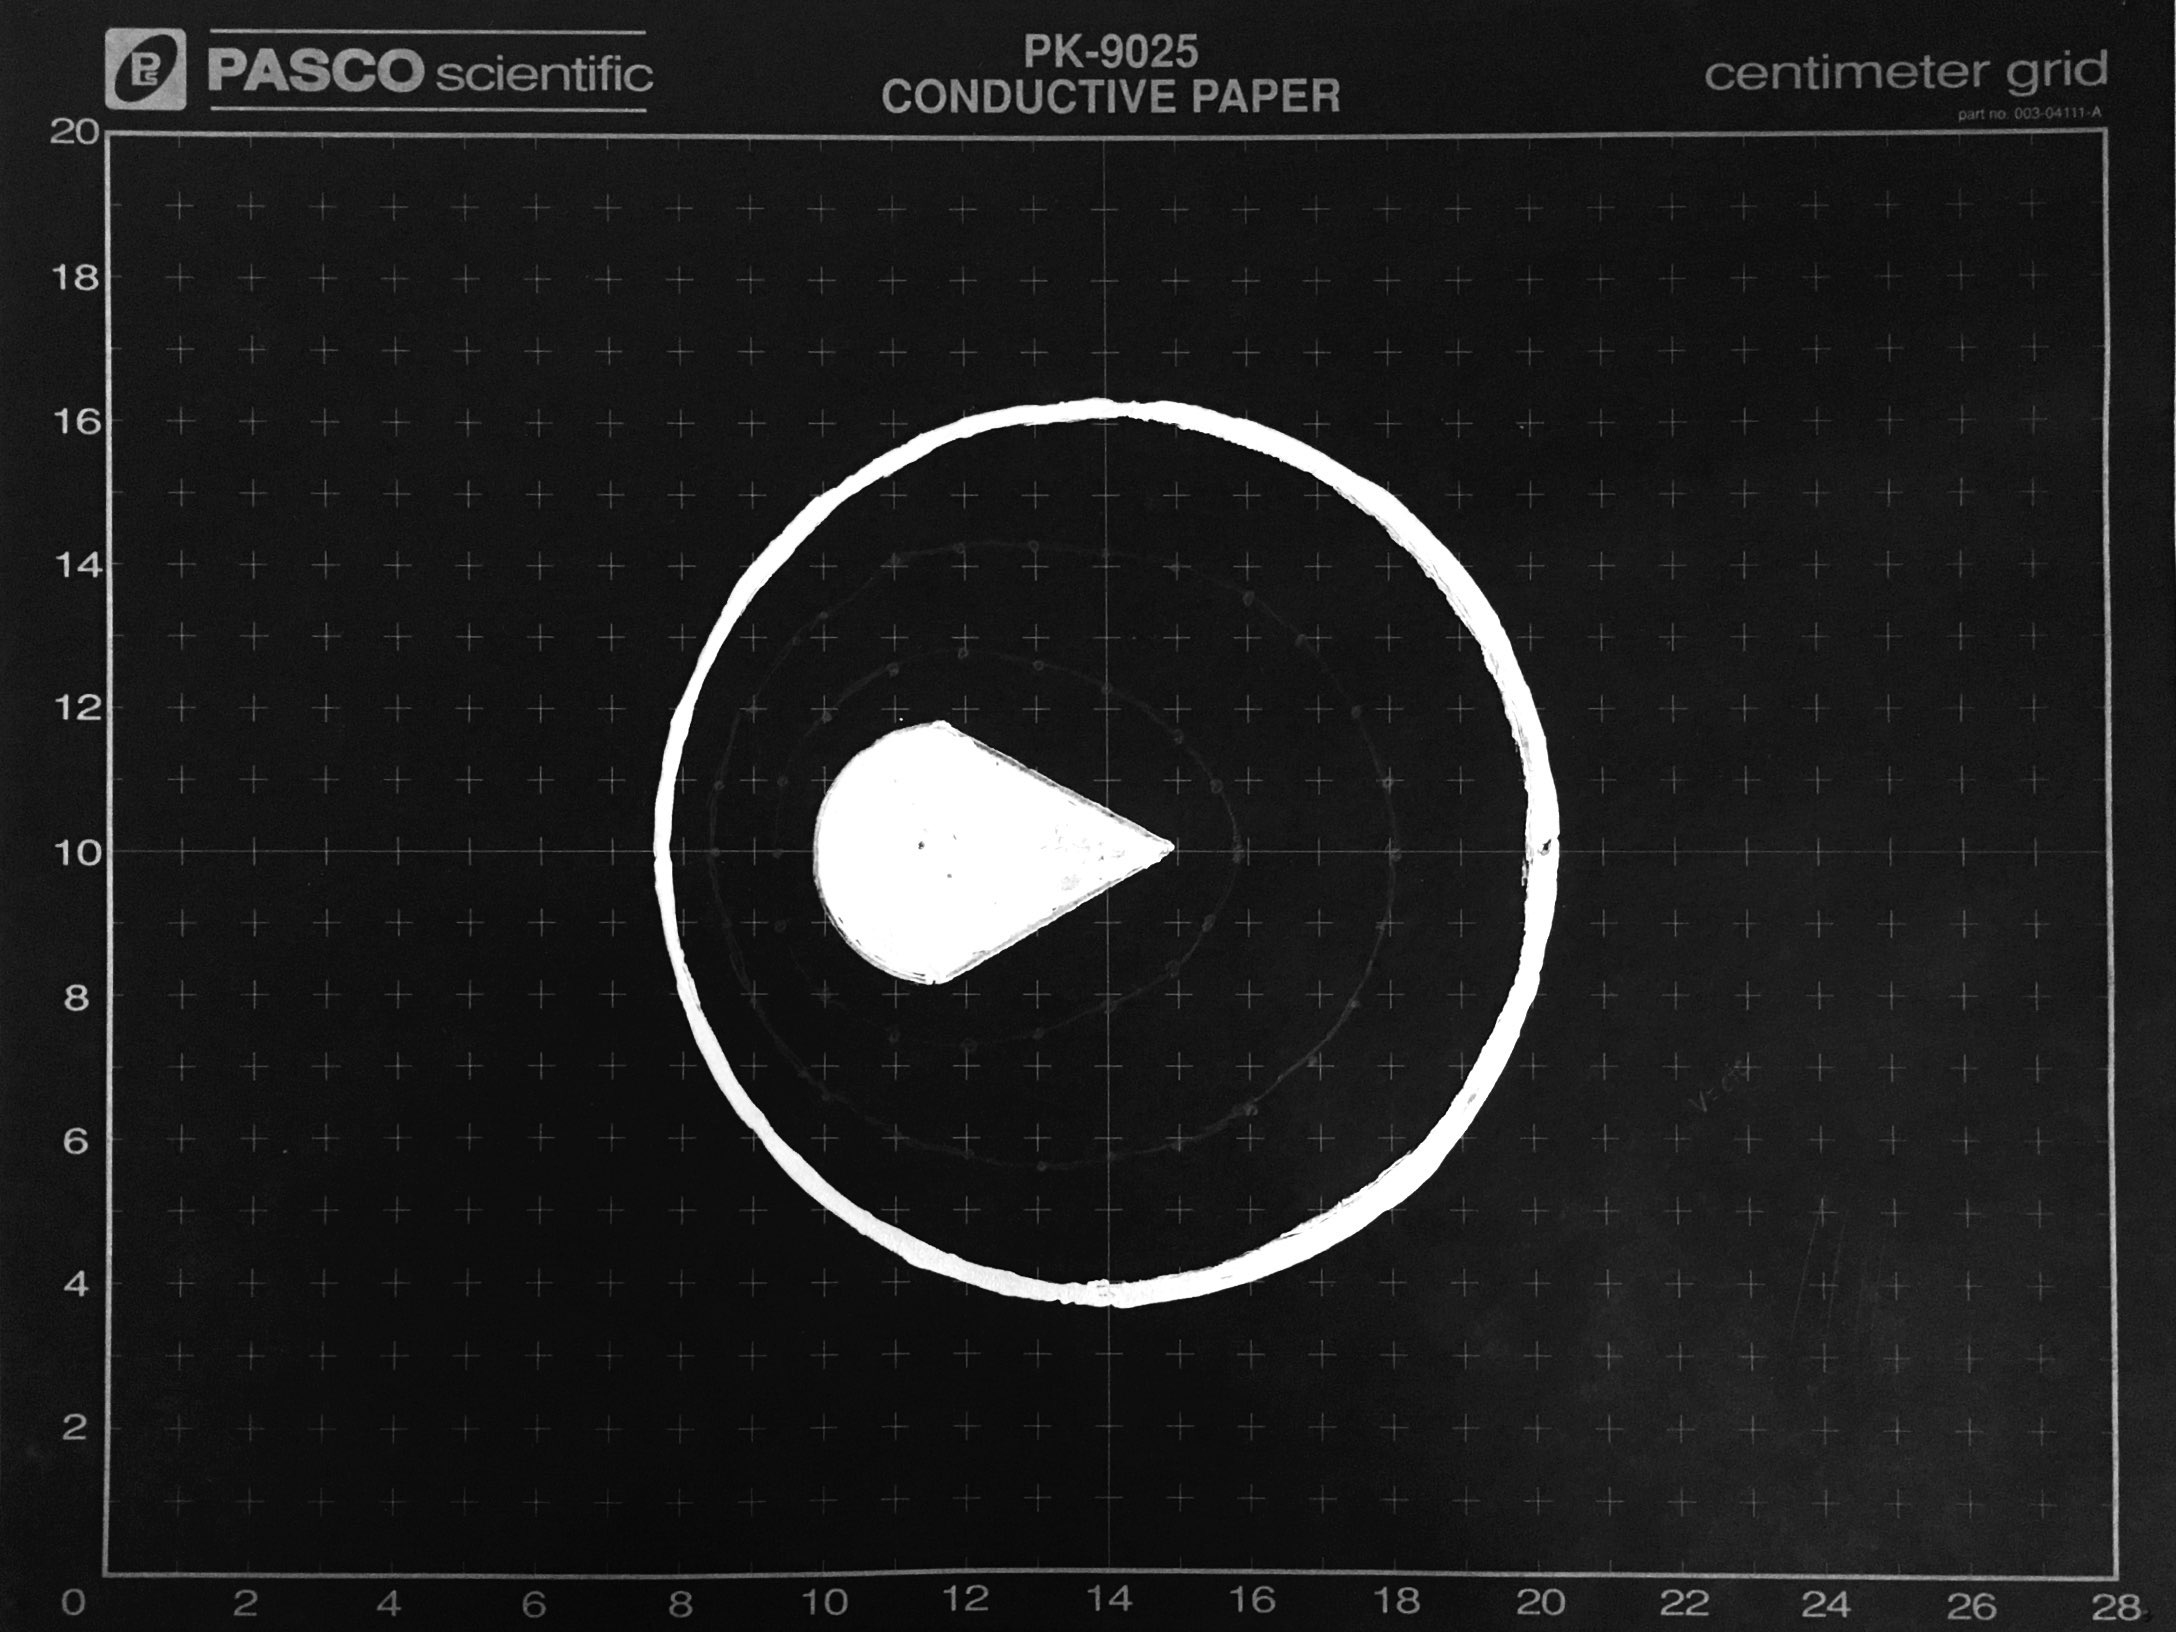
\includegraphics[scale=0.1]{carbo-lliure.jpg}
  \caption{Paper de carbó corresponent a la distribució lliure}
  \label{fig:carbo lliure}
\end{figure}

\subsection{Condensador}
\begin{figure}[htb]
  \centering \small \sffamily
  % GNUPLOT: LaTeX picture with Postscript
\begingroup
  \makeatletter
  \providecommand\color[2][]{%
    \GenericError{(gnuplot) \space\space\space\@spaces}{%
      Package color not loaded in conjunction with
      terminal option `colourtext'%
    }{See the gnuplot documentation for explanation.%
    }{Either use 'blacktext' in gnuplot or load the package
      color.sty in LaTeX.}%
    \renewcommand\color[2][]{}%
  }%
  \providecommand\includegraphics[2][]{%
    \GenericError{(gnuplot) \space\space\space\@spaces}{%
      Package graphicx or graphics not loaded%
    }{See the gnuplot documentation for explanation.%
    }{The gnuplot epslatex terminal needs graphicx.sty or graphics.sty.}%
    \renewcommand\includegraphics[2][]{}%
  }%
  \providecommand\rotatebox[2]{#2}%
  \@ifundefined{ifGPcolor}{%
    \newif\ifGPcolor
    \GPcolortrue
  }{}%
  \@ifundefined{ifGPblacktext}{%
    \newif\ifGPblacktext
    \GPblacktextfalse
  }{}%
  % define a \g@addto@macro without @ in the name:
  \let\gplgaddtomacro\g@addto@macro
  % define empty templates for all commands taking text:
  \gdef\gplbacktext{}%
  \gdef\gplfronttext{}%
  \makeatother
  \ifGPblacktext
    % no textcolor at all
    \def\colorrgb#1{}%
    \def\colorgray#1{}%
  \else
    % gray or color?
    \ifGPcolor
      \def\colorrgb#1{\color[rgb]{#1}}%
      \def\colorgray#1{\color[gray]{#1}}%
      \expandafter\def\csname LTw\endcsname{\color{white}}%
      \expandafter\def\csname LTb\endcsname{\color{black}}%
      \expandafter\def\csname LTa\endcsname{\color{black}}%
      \expandafter\def\csname LT0\endcsname{\color[rgb]{1,0,0}}%
      \expandafter\def\csname LT1\endcsname{\color[rgb]{0,1,0}}%
      \expandafter\def\csname LT2\endcsname{\color[rgb]{0,0,1}}%
      \expandafter\def\csname LT3\endcsname{\color[rgb]{1,0,1}}%
      \expandafter\def\csname LT4\endcsname{\color[rgb]{0,1,1}}%
      \expandafter\def\csname LT5\endcsname{\color[rgb]{1,1,0}}%
      \expandafter\def\csname LT6\endcsname{\color[rgb]{0,0,0}}%
      \expandafter\def\csname LT7\endcsname{\color[rgb]{1,0.3,0}}%
      \expandafter\def\csname LT8\endcsname{\color[rgb]{0.5,0.5,0.5}}%
    \else
      % gray
      \def\colorrgb#1{\color{black}}%
      \def\colorgray#1{\color[gray]{#1}}%
      \expandafter\def\csname LTw\endcsname{\color{white}}%
      \expandafter\def\csname LTb\endcsname{\color{black}}%
      \expandafter\def\csname LTa\endcsname{\color{black}}%
      \expandafter\def\csname LT0\endcsname{\color{black}}%
      \expandafter\def\csname LT1\endcsname{\color{black}}%
      \expandafter\def\csname LT2\endcsname{\color{black}}%
      \expandafter\def\csname LT3\endcsname{\color{black}}%
      \expandafter\def\csname LT4\endcsname{\color{black}}%
      \expandafter\def\csname LT5\endcsname{\color{black}}%
      \expandafter\def\csname LT6\endcsname{\color{black}}%
      \expandafter\def\csname LT7\endcsname{\color{black}}%
      \expandafter\def\csname LT8\endcsname{\color{black}}%
    \fi
  \fi
    \setlength{\unitlength}{0.0500bp}%
    \ifx\gptboxheight\undefined%
      \newlength{\gptboxheight}%
      \newlength{\gptboxwidth}%
      \newsavebox{\gptboxtext}%
    \fi%
    \setlength{\fboxrule}{0.5pt}%
    \setlength{\fboxsep}{1pt}%
\begin{picture}(5668.00,5668.00)%
    \gplgaddtomacro\gplbacktext{%
    }%
    \gplgaddtomacro\gplfronttext{%
      \csname LTb\endcsname%%
      \put(793,690){\makebox(0,0){\strut{}\num{0}}}%
      \put(1522,690){\makebox(0,0){\strut{}\num{50}}}%
      \put(2251,690){\makebox(0,0){\strut{}\num{100}}}%
      \put(2979,690){\makebox(0,0){\strut{}\num{150}}}%
      \put(3708,690){\makebox(0,0){\strut{}\num{200}}}%
      \put(4437,690){\makebox(0,0){\strut{}\num{250}}}%
      \put(2834,360){\makebox(0,0){\strut{}$x$ (\si{mm})}}%
      \put(601,1304){\makebox(0,0)[r]{\strut{}\num{20}}}%
      \put(601,1714){\makebox(0,0)[r]{\strut{}\num{40}}}%
      \put(601,2124){\makebox(0,0)[r]{\strut{}\num{60}}}%
      \put(601,2534){\makebox(0,0)[r]{\strut{}\num{80}}}%
      \put(601,2944){\makebox(0,0)[r]{\strut{}\num{100}}}%
      \put(601,3354){\makebox(0,0)[r]{\strut{}\num{120}}}%
      \put(601,3764){\makebox(0,0)[r]{\strut{}\num{140}}}%
      \put(601,4174){\makebox(0,0)[r]{\strut{}\num{160}}}%
      \put(601,4584){\makebox(0,0)[r]{\strut{}\num{180}}}%
      \put(7,2944){\rotatebox{-270}{\makebox(0,0){\strut{}$y$ (\si{mm})}}}%
      \put(5313,997){\makebox(0,0)[l]{\strut{}\num{-1}}}%
      \put(5313,1970){\makebox(0,0)[l]{\strut{}\num{-0.5}}}%
      \put(5313,2944){\makebox(0,0)[l]{\strut{}\num{0}}}%
      \put(5313,3917){\makebox(0,0)[l]{\strut{}\num{0.5}}}%
      \put(5313,4891){\makebox(0,0)[l]{\strut{}\num{1}}}%
    }%
    \gplbacktext
    \put(0,0){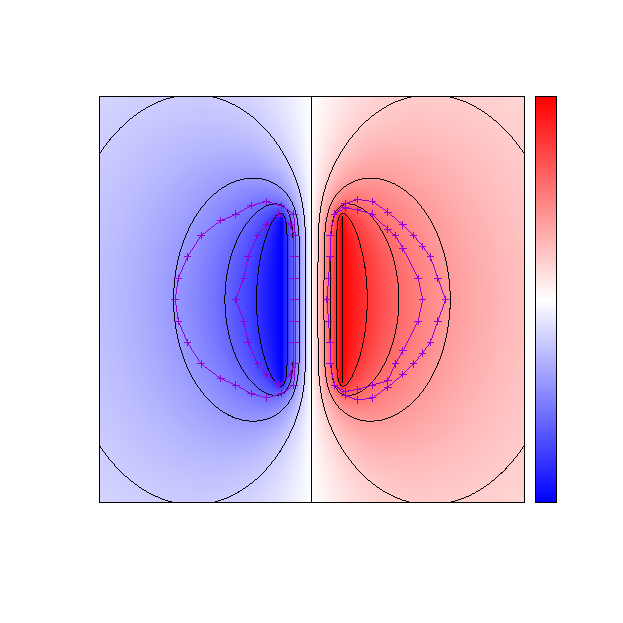
\includegraphics{condensador}}%
    \gplfronttext
  \end{picture}%
\endgroup

  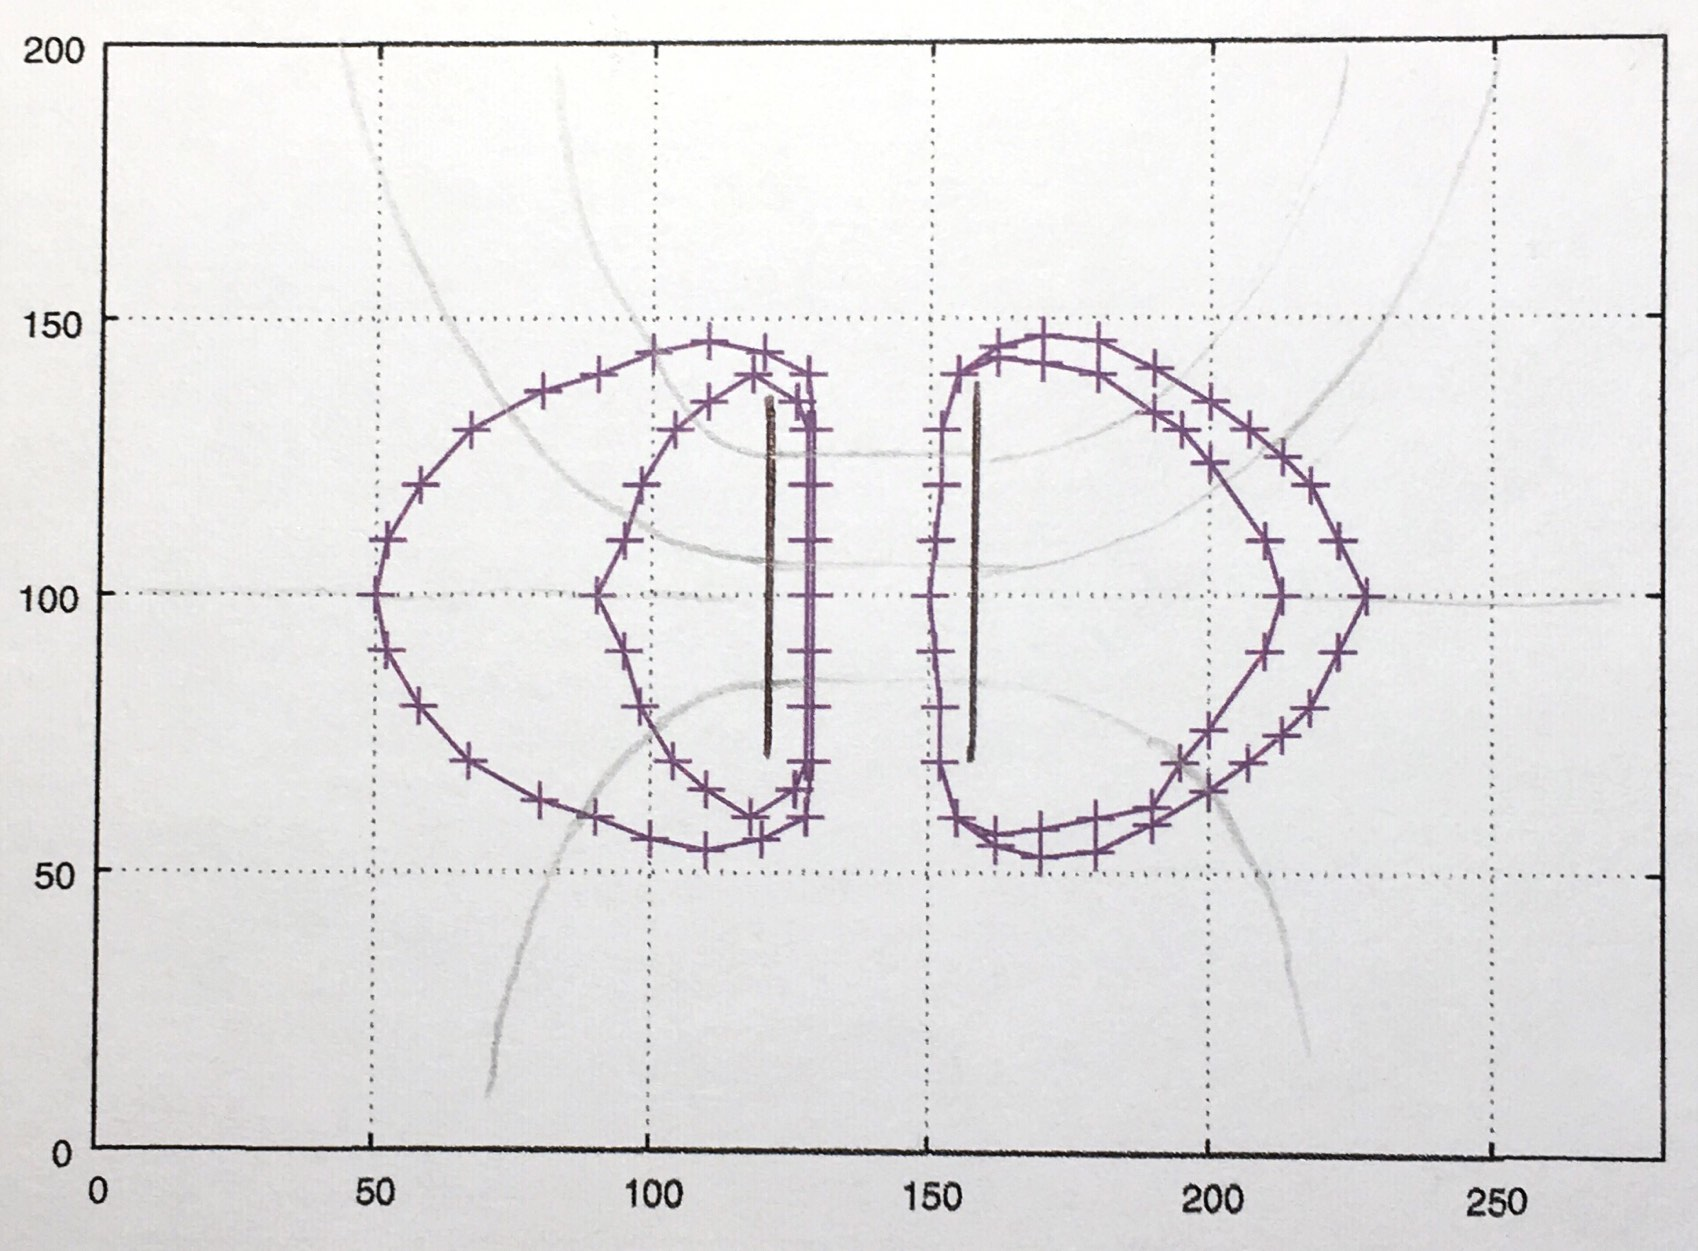
\includegraphics[scale=0.5]{condensador-campexp.jpg}
  \caption{a)Punts experimentals trobats per al condensador, amb les línies equipotencials experimentals i teòriques
  b) Línies de camp experimentals}
  \label{fig:camp condensador}
\end{figure}

La nostra primera mesura és la dels dos condensadors plano-para\l.lels de longitud suposadament infinita i densitat superficial de càrrega uniforme. Fixant una diferència de potencial entre les plaques, vam ser capaços de mesurar diferents línies equipotencials, representades a la \cref{fig:camp condensador}, tant les experimentals com les teòriques. Així mateix, vam esbossar com serien les línies de camp.

Es pot veure que en forma són força semblants, la qual cosa garanteix el bon resultat obtingut. A més, cal afegir que aquest condensador només és infinit a la coordenada $z$, mentre que és finit a la $y$. Per a punts allunyats de la vora, les línies de camp són pràcticament perpendiculars, igual que les aproximacions fetes normalment. Però a la vora hi ha un ràpid creixement i les línies perden el seu caràcter recte.

D'altra banda, d'aquesta distribució pretenem també obtenir una expressió de la capacitat per unitat de longitud. Per a aconseguir-ho, farem ús de l'equació \cref{eq:carrega} per a obtenir una expressió de la càrrega en funció de la longitud de la placa del condensador. Cal dir que les distàncies presentaven una incertesa d'origen instrumental de $ \data{}{1}{mm} $, però això es complicava més quan havíem de mesurar $\Delta l_i$, ja que eren línies corbes. Això és una possible font d'error. Per a reduir-la, vam prendre moltes mesures molt properes, de manera que els arcs de corba fossin aproximadament com cordes, és a dir, com rectes. L'incertesa associada a $Q/Z$ combina les incerteses de les altres tres magnituds.

La capacitat promig és llavors $C/\epsilon = \data{1.6}{0.4}{F.m^{-1}}$. Podem calcular també el seu valor teòric, aplicant l'equació \cref{eq:capacitat 2}, i substituint els valors de separació i longitud de les plaques, deixant la permitivitat com a constant desconeguda.
Així s'obté un valor teòric de $C_T/\epsilon = \data{2.0}{0.1}{F.m^{-1}} $. Com podem veure, totes dues mesures són compatibles degut a l'incertesa de l'experimental. També presenten un error relatiu petit, del $20\%$. Sembla llavors una bona estimació.

\subsection{Fils para\l.lels}
\begin{figure}[htb]
  \centering \small \sffamily
	% GNUPLOT: LaTeX picture with Postscript
\begingroup
  \makeatletter
  \providecommand\color[2][]{%
    \GenericError{(gnuplot) \space\space\space\@spaces}{%
      Package color not loaded in conjunction with
      terminal option `colourtext'%
    }{See the gnuplot documentation for explanation.%
    }{Either use 'blacktext' in gnuplot or load the package
      color.sty in LaTeX.}%
    \renewcommand\color[2][]{}%
  }%
  \providecommand\includegraphics[2][]{%
    \GenericError{(gnuplot) \space\space\space\@spaces}{%
      Package graphicx or graphics not loaded%
    }{See the gnuplot documentation for explanation.%
    }{The gnuplot epslatex terminal needs graphicx.sty or graphics.sty.}%
    \renewcommand\includegraphics[2][]{}%
  }%
  \providecommand\rotatebox[2]{#2}%
  \@ifundefined{ifGPcolor}{%
    \newif\ifGPcolor
    \GPcolortrue
  }{}%
  \@ifundefined{ifGPblacktext}{%
    \newif\ifGPblacktext
    \GPblacktextfalse
  }{}%
  % define a \g@addto@macro without @ in the name:
  \let\gplgaddtomacro\g@addto@macro
  % define empty templates for all commands taking text:
  \gdef\gplbacktext{}%
  \gdef\gplfronttext{}%
  \makeatother
  \ifGPblacktext
    % no textcolor at all
    \def\colorrgb#1{}%
    \def\colorgray#1{}%
  \else
    % gray or color?
    \ifGPcolor
      \def\colorrgb#1{\color[rgb]{#1}}%
      \def\colorgray#1{\color[gray]{#1}}%
      \expandafter\def\csname LTw\endcsname{\color{white}}%
      \expandafter\def\csname LTb\endcsname{\color{black}}%
      \expandafter\def\csname LTa\endcsname{\color{black}}%
      \expandafter\def\csname LT0\endcsname{\color[rgb]{1,0,0}}%
      \expandafter\def\csname LT1\endcsname{\color[rgb]{0,1,0}}%
      \expandafter\def\csname LT2\endcsname{\color[rgb]{0,0,1}}%
      \expandafter\def\csname LT3\endcsname{\color[rgb]{1,0,1}}%
      \expandafter\def\csname LT4\endcsname{\color[rgb]{0,1,1}}%
      \expandafter\def\csname LT5\endcsname{\color[rgb]{1,1,0}}%
      \expandafter\def\csname LT6\endcsname{\color[rgb]{0,0,0}}%
      \expandafter\def\csname LT7\endcsname{\color[rgb]{1,0.3,0}}%
      \expandafter\def\csname LT8\endcsname{\color[rgb]{0.5,0.5,0.5}}%
    \else
      % gray
      \def\colorrgb#1{\color{black}}%
      \def\colorgray#1{\color[gray]{#1}}%
      \expandafter\def\csname LTw\endcsname{\color{white}}%
      \expandafter\def\csname LTb\endcsname{\color{black}}%
      \expandafter\def\csname LTa\endcsname{\color{black}}%
      \expandafter\def\csname LT0\endcsname{\color{black}}%
      \expandafter\def\csname LT1\endcsname{\color{black}}%
      \expandafter\def\csname LT2\endcsname{\color{black}}%
      \expandafter\def\csname LT3\endcsname{\color{black}}%
      \expandafter\def\csname LT4\endcsname{\color{black}}%
      \expandafter\def\csname LT5\endcsname{\color{black}}%
      \expandafter\def\csname LT6\endcsname{\color{black}}%
      \expandafter\def\csname LT7\endcsname{\color{black}}%
      \expandafter\def\csname LT8\endcsname{\color{black}}%
    \fi
  \fi
    \setlength{\unitlength}{0.0500bp}%
    \ifx\gptboxheight\undefined%
      \newlength{\gptboxheight}%
      \newlength{\gptboxwidth}%
      \newsavebox{\gptboxtext}%
    \fi%
    \setlength{\fboxrule}{0.5pt}%
    \setlength{\fboxsep}{1pt}%
\begin{picture}(5668.00,5668.00)%
    \gplgaddtomacro\gplbacktext{%
    }%
    \gplgaddtomacro\gplfronttext{%
    }%
    \gplbacktext
    \put(0,0){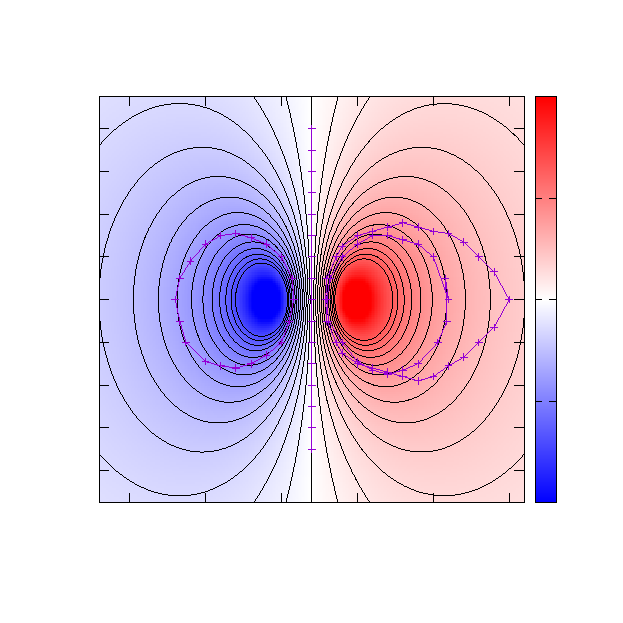
\includegraphics{fils}}%
    \gplfronttext
  \end{picture}%
\endgroup

	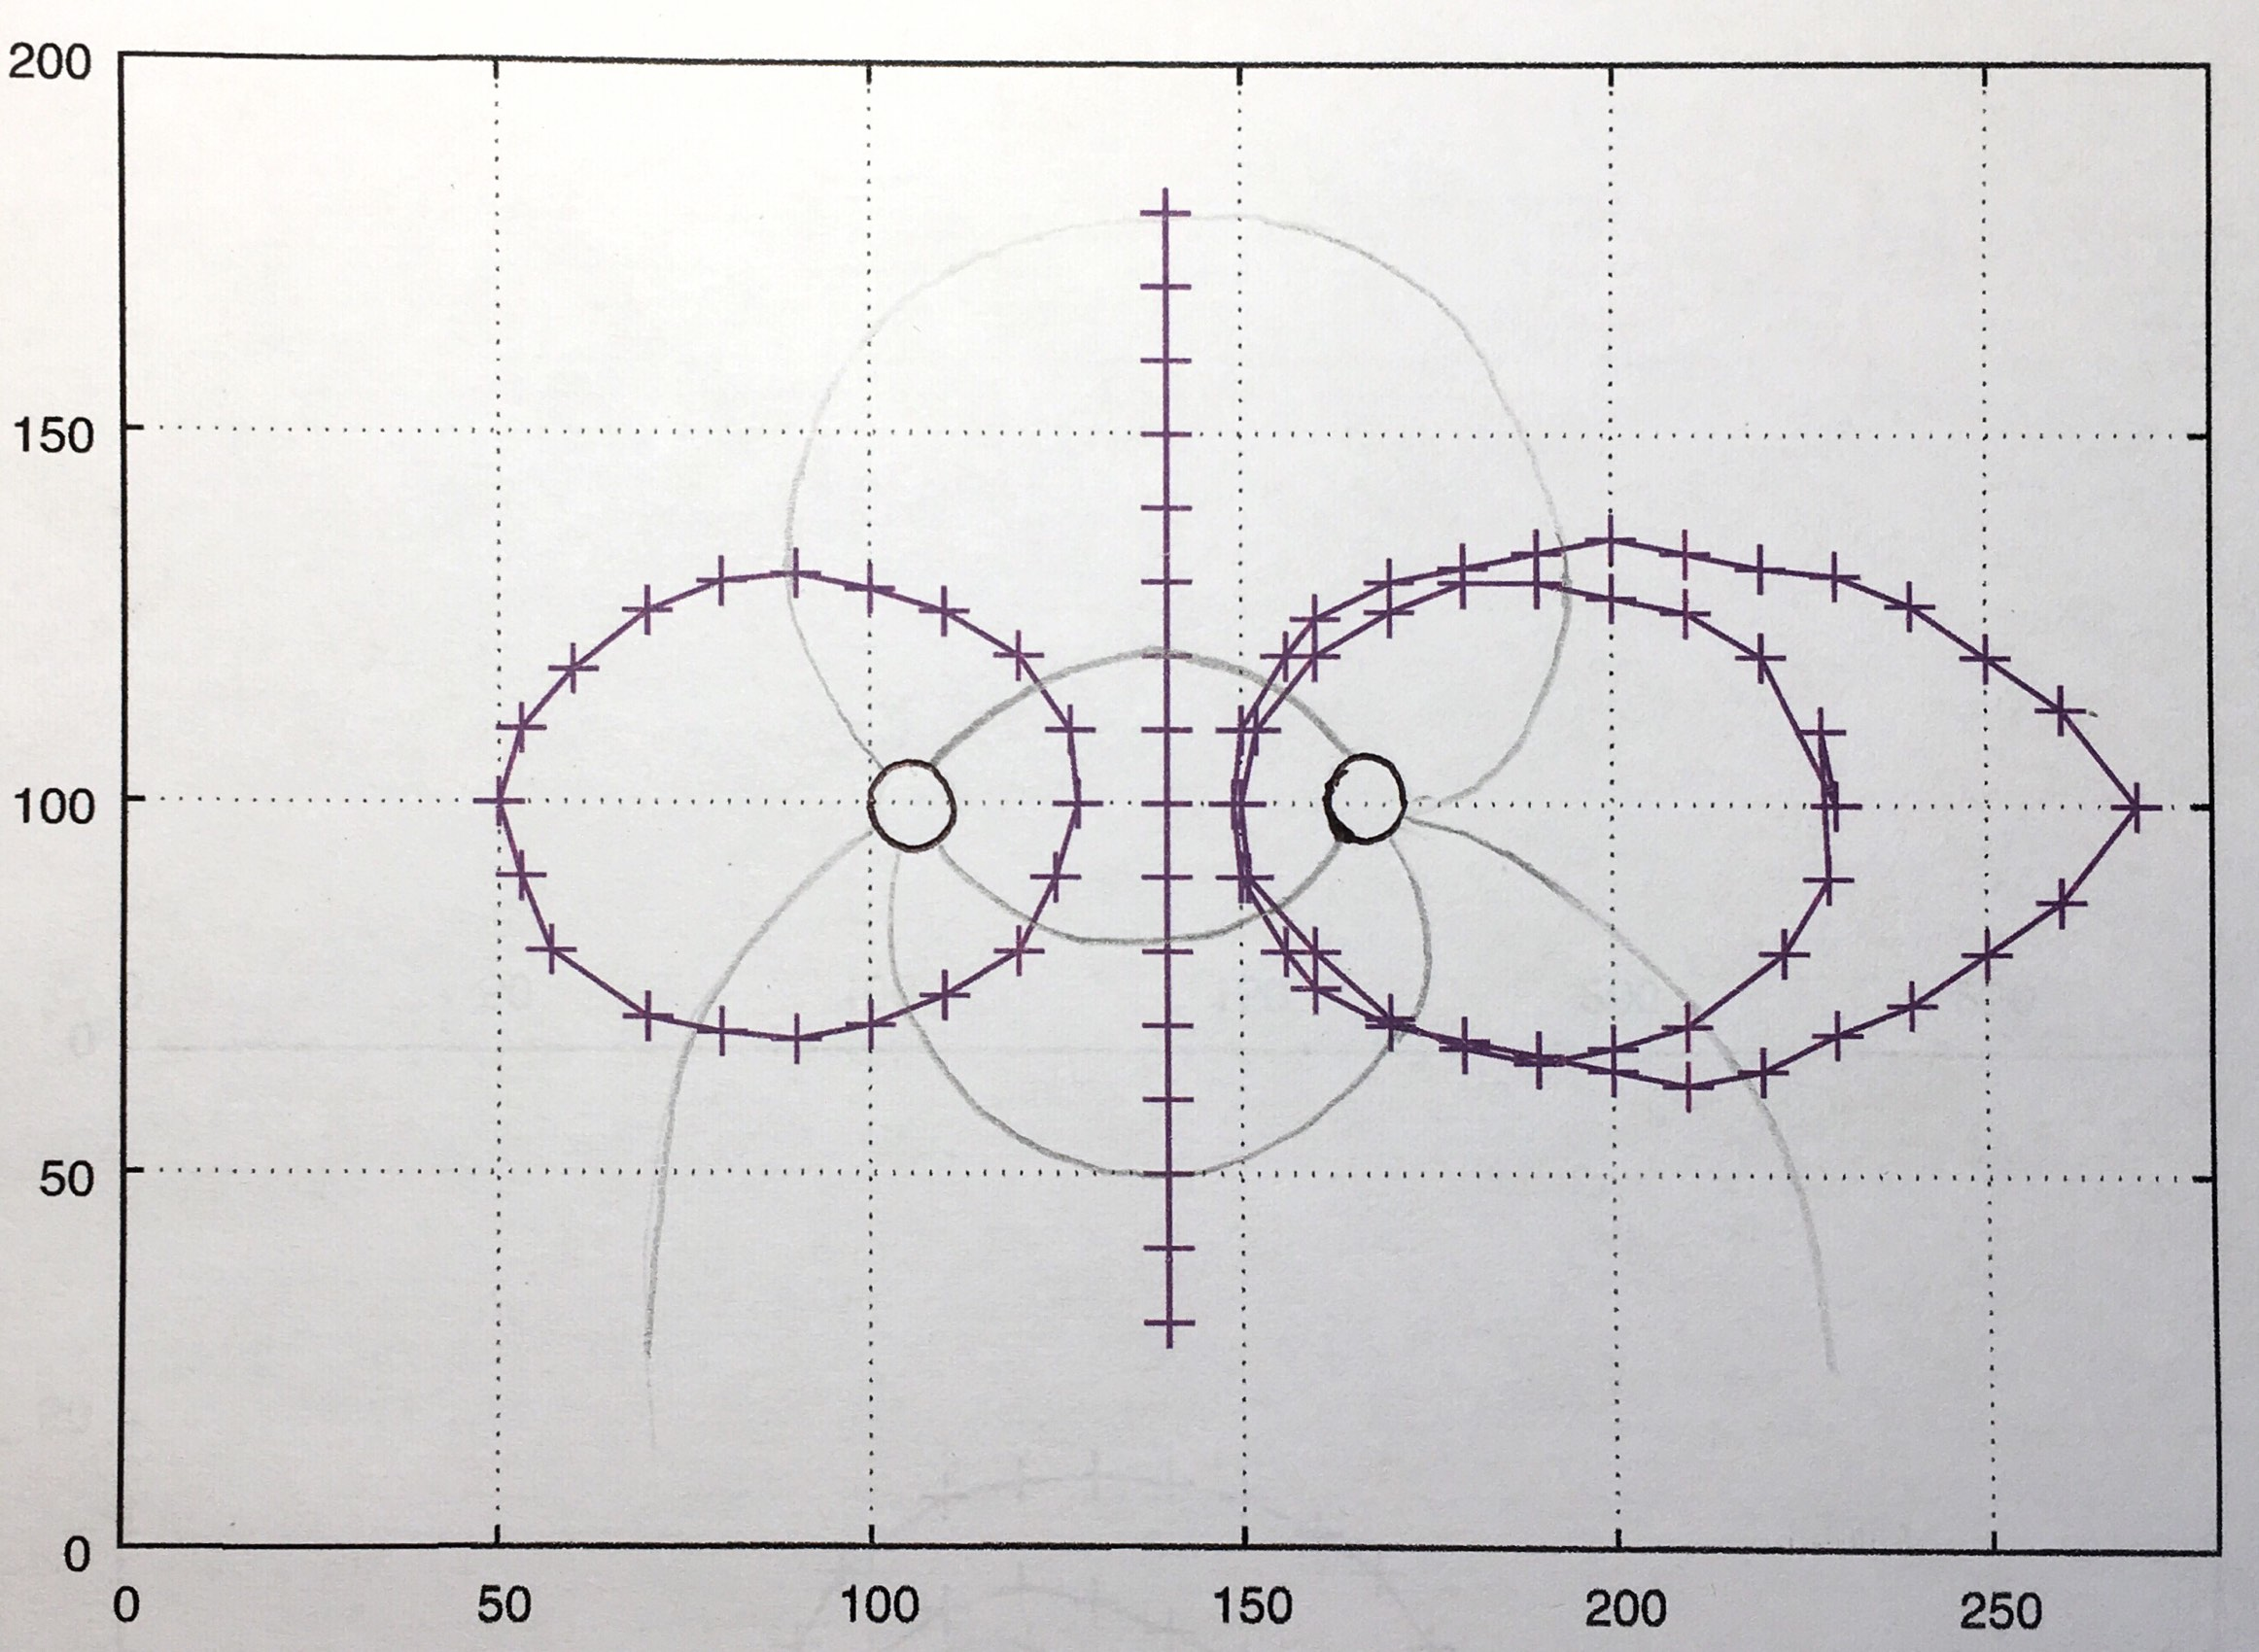
\includegraphics[scale=0.5]{hilos-campexp.jpg}
  \caption{a) Punts experimentals trobats per als fils para\l.lels, amb les línies equipotencials experimentals i teòriques
  b) Línies de camp experimentals}
  \label{fig:camp fils}
\end{figure}

La segona distribució de càrrega que vam analitzar va ser la de dos fils o cables infinits. De nou, tenim la secció corresponent a una intersecció amb un pla perpendicular als dos. Idealment només es veurien dos punts de plata, però els fem una mica gruixuts (tots dos amb el mateix radi) per a poder realitzar millor les mesures. Un altre cop vam fixar la diferència de potencial entre els fils i vam procedir a mesurar. Les línies equipotencials i de camp es poden veure a la \cref{fig:camp fils}. Tenim que en forma són molt semblants la teórica i l'experimental.

\subsection{Distribució lliure}
\begin{figure}[htb]
  \centering \small \sffamily
	% GNUPLOT: LaTeX picture with Postscript
\begingroup
  \makeatletter
  \providecommand\color[2][]{%
    \GenericError{(gnuplot) \space\space\space\@spaces}{%
      Package color not loaded in conjunction with
      terminal option `colourtext'%
    }{See the gnuplot documentation for explanation.%
    }{Either use 'blacktext' in gnuplot or load the package
      color.sty in LaTeX.}%
    \renewcommand\color[2][]{}%
  }%
  \providecommand\includegraphics[2][]{%
    \GenericError{(gnuplot) \space\space\space\@spaces}{%
      Package graphicx or graphics not loaded%
    }{See the gnuplot documentation for explanation.%
    }{The gnuplot epslatex terminal needs graphicx.sty or graphics.sty.}%
    \renewcommand\includegraphics[2][]{}%
  }%
  \providecommand\rotatebox[2]{#2}%
  \@ifundefined{ifGPcolor}{%
    \newif\ifGPcolor
    \GPcolortrue
  }{}%
  \@ifundefined{ifGPblacktext}{%
    \newif\ifGPblacktext
    \GPblacktextfalse
  }{}%
  % define a \g@addto@macro without @ in the name:
  \let\gplgaddtomacro\g@addto@macro
  % define empty templates for all commands taking text:
  \gdef\gplbacktext{}%
  \gdef\gplfronttext{}%
  \makeatother
  \ifGPblacktext
    % no textcolor at all
    \def\colorrgb#1{}%
    \def\colorgray#1{}%
  \else
    % gray or color?
    \ifGPcolor
      \def\colorrgb#1{\color[rgb]{#1}}%
      \def\colorgray#1{\color[gray]{#1}}%
      \expandafter\def\csname LTw\endcsname{\color{white}}%
      \expandafter\def\csname LTb\endcsname{\color{black}}%
      \expandafter\def\csname LTa\endcsname{\color{black}}%
      \expandafter\def\csname LT0\endcsname{\color[rgb]{1,0,0}}%
      \expandafter\def\csname LT1\endcsname{\color[rgb]{0,1,0}}%
      \expandafter\def\csname LT2\endcsname{\color[rgb]{0,0,1}}%
      \expandafter\def\csname LT3\endcsname{\color[rgb]{1,0,1}}%
      \expandafter\def\csname LT4\endcsname{\color[rgb]{0,1,1}}%
      \expandafter\def\csname LT5\endcsname{\color[rgb]{1,1,0}}%
      \expandafter\def\csname LT6\endcsname{\color[rgb]{0,0,0}}%
      \expandafter\def\csname LT7\endcsname{\color[rgb]{1,0.3,0}}%
      \expandafter\def\csname LT8\endcsname{\color[rgb]{0.5,0.5,0.5}}%
    \else
      % gray
      \def\colorrgb#1{\color{black}}%
      \def\colorgray#1{\color[gray]{#1}}%
      \expandafter\def\csname LTw\endcsname{\color{white}}%
      \expandafter\def\csname LTb\endcsname{\color{black}}%
      \expandafter\def\csname LTa\endcsname{\color{black}}%
      \expandafter\def\csname LT0\endcsname{\color{black}}%
      \expandafter\def\csname LT1\endcsname{\color{black}}%
      \expandafter\def\csname LT2\endcsname{\color{black}}%
      \expandafter\def\csname LT3\endcsname{\color{black}}%
      \expandafter\def\csname LT4\endcsname{\color{black}}%
      \expandafter\def\csname LT5\endcsname{\color{black}}%
      \expandafter\def\csname LT6\endcsname{\color{black}}%
      \expandafter\def\csname LT7\endcsname{\color{black}}%
      \expandafter\def\csname LT8\endcsname{\color{black}}%
    \fi
  \fi
    \setlength{\unitlength}{0.0500bp}%
    \ifx\gptboxheight\undefined%
      \newlength{\gptboxheight}%
      \newlength{\gptboxwidth}%
      \newsavebox{\gptboxtext}%
    \fi%
    \setlength{\fboxrule}{0.5pt}%
    \setlength{\fboxsep}{1pt}%
\begin{picture}(5668.00,5668.00)%
    \gplgaddtomacro\gplbacktext{%
    }%
    \gplgaddtomacro\gplfronttext{%
      \csname LTb\endcsname%%
      \put(793,700){\makebox(0,0){\strut{}\num{50}}}%
      \put(1814,700){\makebox(0,0){\strut{}\num{100}}}%
      \put(2834,700){\makebox(0,0){\strut{}\num{150}}}%
      \put(3854,700){\makebox(0,0){\strut{}\num{200}}}%
      \put(4875,700){\makebox(0,0){\strut{}\num{250}}}%
      \put(2834,370){\makebox(0,0){\strut{}$x$ (\si{mm})}}%
      \put(600,1312){\makebox(0,0)[r]{\strut{}\num{20}}}%
      \put(600,1720){\makebox(0,0)[r]{\strut{}\num{40}}}%
      \put(600,2128){\makebox(0,0)[r]{\strut{}\num{60}}}%
      \put(600,2536){\makebox(0,0)[r]{\strut{}\num{80}}}%
      \put(600,2944){\makebox(0,0)[r]{\strut{}\num{100}}}%
      \put(600,3352){\makebox(0,0)[r]{\strut{}\num{120}}}%
      \put(600,3760){\makebox(0,0)[r]{\strut{}\num{140}}}%
      \put(600,4168){\makebox(0,0)[r]{\strut{}\num{160}}}%
      \put(600,4576){\makebox(0,0)[r]{\strut{}\num{180}}}%
      \put(6,2944){\rotatebox{-270}{\makebox(0,0){\strut{}$y$ (\si{mm})}}}%
      \put(5313,1006){\makebox(0,0)[l]{\strut{}\num{-1}}}%
      \put(5313,1975){\makebox(0,0)[l]{\strut{}\num{-0.5}}}%
      \put(5313,2944){\makebox(0,0)[l]{\strut{}\num{0}}}%
      \put(5313,3913){\makebox(0,0)[l]{\strut{}\num{0.5}}}%
      \put(5313,4882){\makebox(0,0)[l]{\strut{}\num{1}}}%
    }%
    \gplbacktext
    \put(0,0){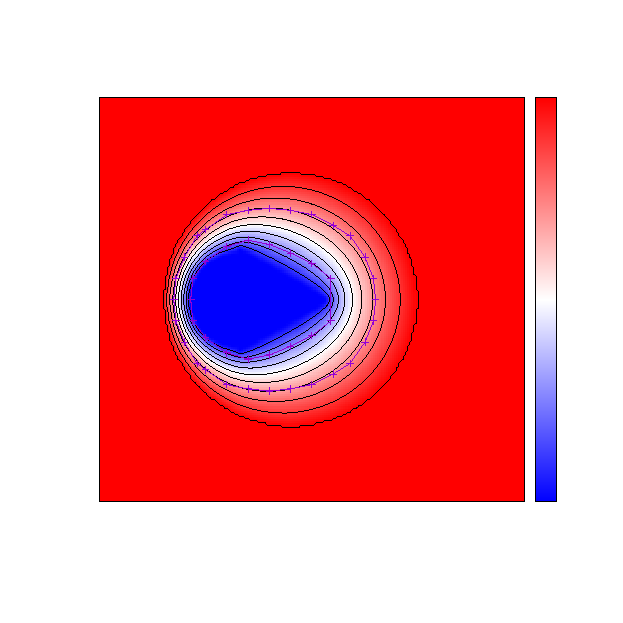
\includegraphics{lliure}}%
    \gplfronttext
  \end{picture}%
\endgroup

	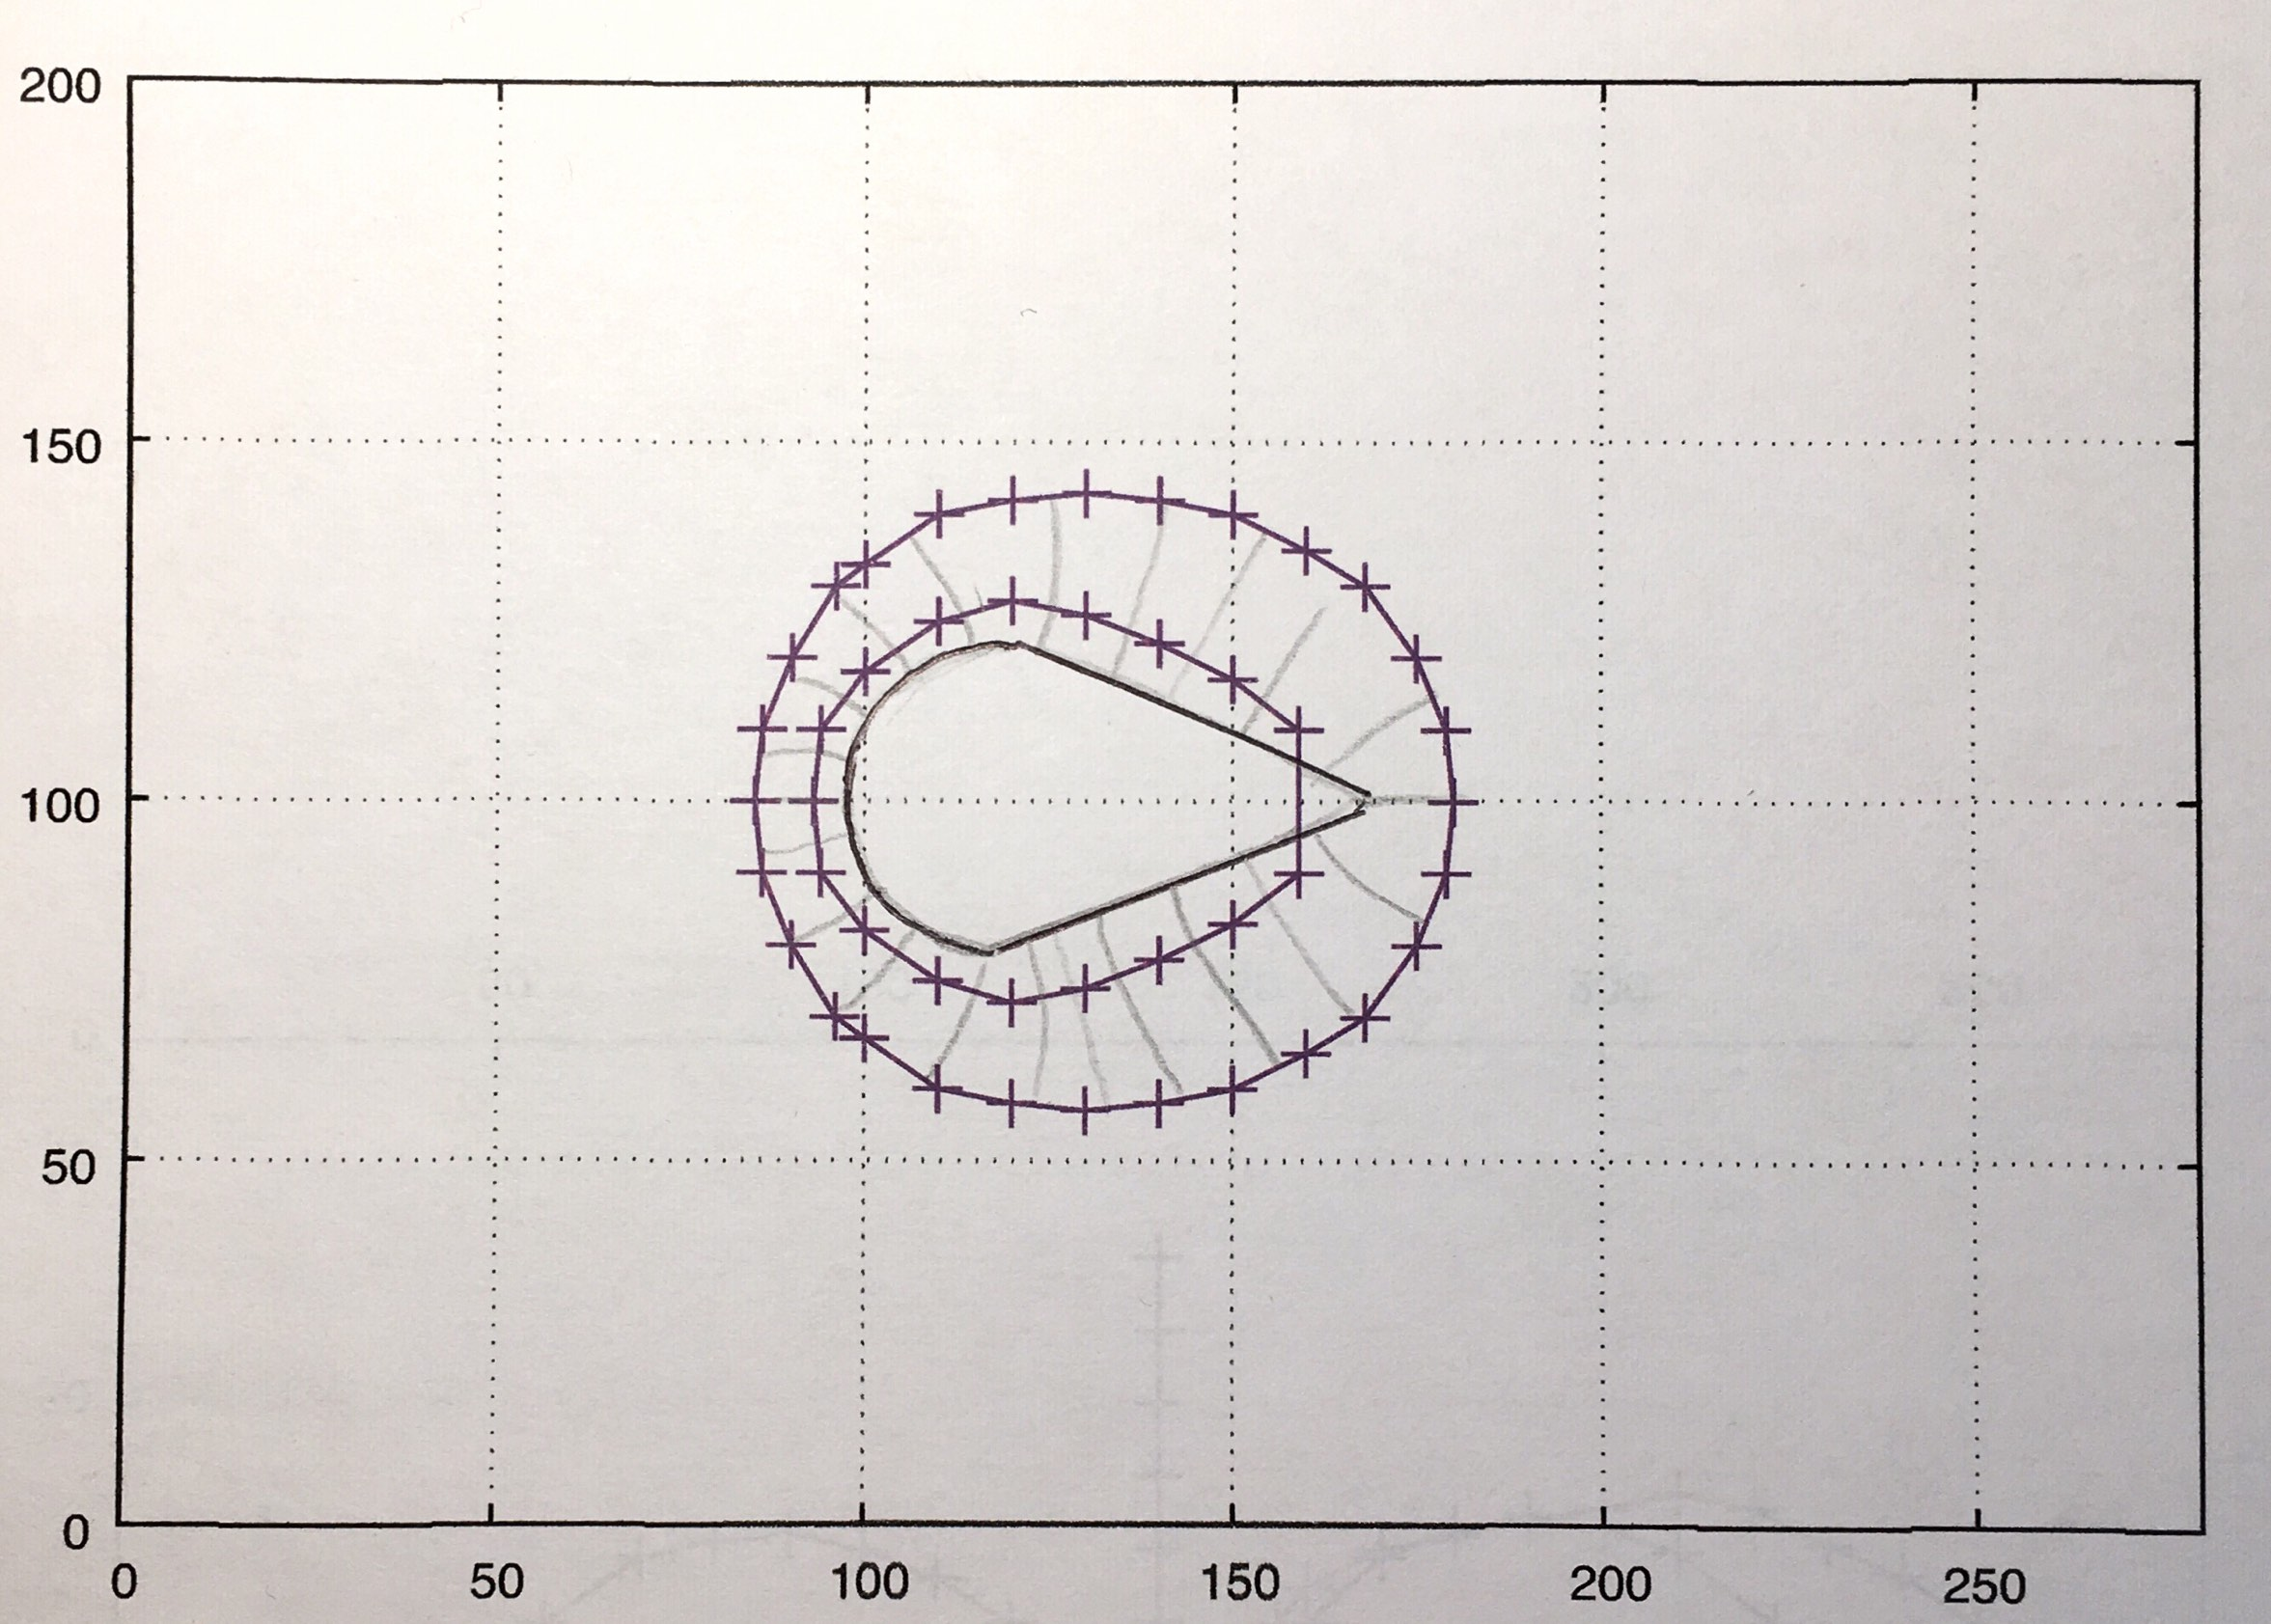
\includegraphics[scale=0.5]{libre-campexp.jpg}
  \caption{a) Punts experimentals trobats per a la distribució lliure, amb les línies equipotencials experimentals i teòriques
  b)Línies de camp experimentals}
  \label{fig:camp lliure}
\end{figure}

Per a aquesta última distribució tractarem d'avaluar el pes de l'efecte punxa en una distribució tancada per una escorça esfèrica. Observant la \cref{fig:carbo condensador}, veiem que la distribució lliure presenta simetria respecte de l'eix $x$. Recordem a més que el mencionat efecte relaciona el camp a la superfície d'un conductor amb el seu radi de curvatura, d'acord amb l'\cref{eq:efecte punxa}, on $E_i$ representa el camp elèctric a la superfície i $r_i$ el radi de curvatura d'aquesta superfície
\begin{equation} \label{eq:efecte punxa}
	E_1r_1=E_2r_2
\end{equation}
de manera que a mesura que el radi decreix, el camp en aquesta part augmenta, esdevenint molt intens en cas que hi hagi punxes.

Per a comprovar aquest efecte, vam provar de dibuixar una figura amb dos radis de curvatura ben diferenciats. Si no existeix l'escorça circular, aquest resultat hauria d'haver-se donat fàcilment, però vam tenir el problema de no ser capaços de preveure l'influència que l'escorça té sobre el camp. Com es pot veure a \cref{fig:camp lliure}, resulta que el camp és més intens a la zona amb radi de curvatura més gran, i això és justament el contrari del que volíem veure. Notem que superfícies equipotencials més properes implica un canvi més ràpid del mòdul del camp, i per tant, un camp més intens en poca distància. Tot i això, la distribució s'assembla molt a la teòrica.

Així doncs no podem estudiar l'efecte punxa. Però sí que podem comentar coses per a investigacions posteriors. Una possible millora seria la reducció de les dimensions del cos interior amb respecte de l'escorça esfèrica que l'envolta, o bé aconseguir una millor proporció de les distàncies als extrems del cos interior. Si ens hi fixem, al nostre cas l'extrem de radi menor és a només un centímetre del centre de l'escorça, mentre que l'altre és a quatre centímetres. La solució potser consisteix en col·locar els dos extrems a la mateixa distància, i reduir les dimensions en general.

\section{Conclusions}
Hem obtingut les línies equipotencials generades per un condensador de plaques plano-para\l.leles i dos fils infinits també para\l.lels. La seva forma és similar a l'obtinguda amb una simulació la qual els calcula a partir de l'expressió analítica. A més, la capacitat per unitat de longitud del nostre condensador és de $C=(1.6\pm0.4)\epsilon F/m$. Té el mateix ordre de magnitud i un valor molt proper al teòric, entrant aquest dins del marge donat per les incerteses.

No vam poder treure però, conclusions satisfactòries sobre l'efecte punxa a la distribució lliure. Tot i això, vam trobar una sèrie de canvis que poden ser de gran ajuda en investigacions posteriors, com són la reducció de les dimensions del cos respecte de l'escorça o la millor disposició espaial del cos dins d'aquesta.

